\documentclass[tikz,border=6pt]{standalone}
\usepackage[T1]{fontenc}
\usepackage[utf8]{inputenc}
\usepackage{helvet}
\renewcommand{\familydefault}{\sfdefault}
\usepackage{siunitx}
\usetikzlibrary{arrows.meta,calc,positioning,shapes.geometric}

\definecolor{Navy}{HTML}{0B1F33}
\definecolor{Ink}{HTML}{183247}
\definecolor{Slate}{HTML}{5D7182}
\definecolor{Line}{HTML}{C7D5DE}
\definecolor{Panel}{HTML}{F5F8FA}
\definecolor{Blue}{HTML}{2678B8}
\definecolor{BlueLight}{HTML}{DCECF7}
\definecolor{Orange}{HTML}{E88932}
\definecolor{OrangeLight}{HTML}{FCE9D6}
\definecolor{Teal}{HTML}{00A7A0}
\definecolor{TealLight}{HTML}{DDF4F1}
\definecolor{Green}{HTML}{5B9E62}
\definecolor{GreenLight}{HTML}{E5F2E6}
\definecolor{Red}{HTML}{C94D4D}
\definecolor{Grey}{HTML}{7D8C97}
\definecolor{GreyLight}{HTML}{E8EEF2}

\tikzset{
  panel/.style={rounded corners=2mm, draw=Line, line width=0.7pt, fill=Panel},
  box/.style={rounded corners=1.2mm, draw=Line, line width=0.7pt, fill=white,
    align=center, inner sep=2.2mm, font=\sffamily\scriptsize},
  reservoir/.style={cylinder, shape border rotate=90, aspect=0.38,
    draw=Navy, line width=0.8pt, align=center, inner sep=1.7mm,
    minimum width=2.05cm, minimum height=1.35cm, font=\sffamily\tiny},
  flow/.style={-{Latex[length=2.5mm,width=1.6mm]}, line width=1.15pt},
  water/.style={-{Latex[length=2.7mm,width=1.8mm]}, line width=1.35pt, Teal},
  waterrev/.style={{Latex[length=2.7mm,width=1.8mm]}-{Latex[length=2.7mm,width=1.8mm]},
    line width=1.35pt, Teal},
  dim/.style={{Bar[width=4pt]}-{Bar[width=4pt]}, line width=0.55pt, Slate},
  leader/.style={line width=0.55pt, Slate},
  note/.style={align=left, font=\sffamily\scriptsize, text=Slate},
  smallnote/.style={align=left, font=\sffamily\tiny, text=Slate}
}

\begin{document}
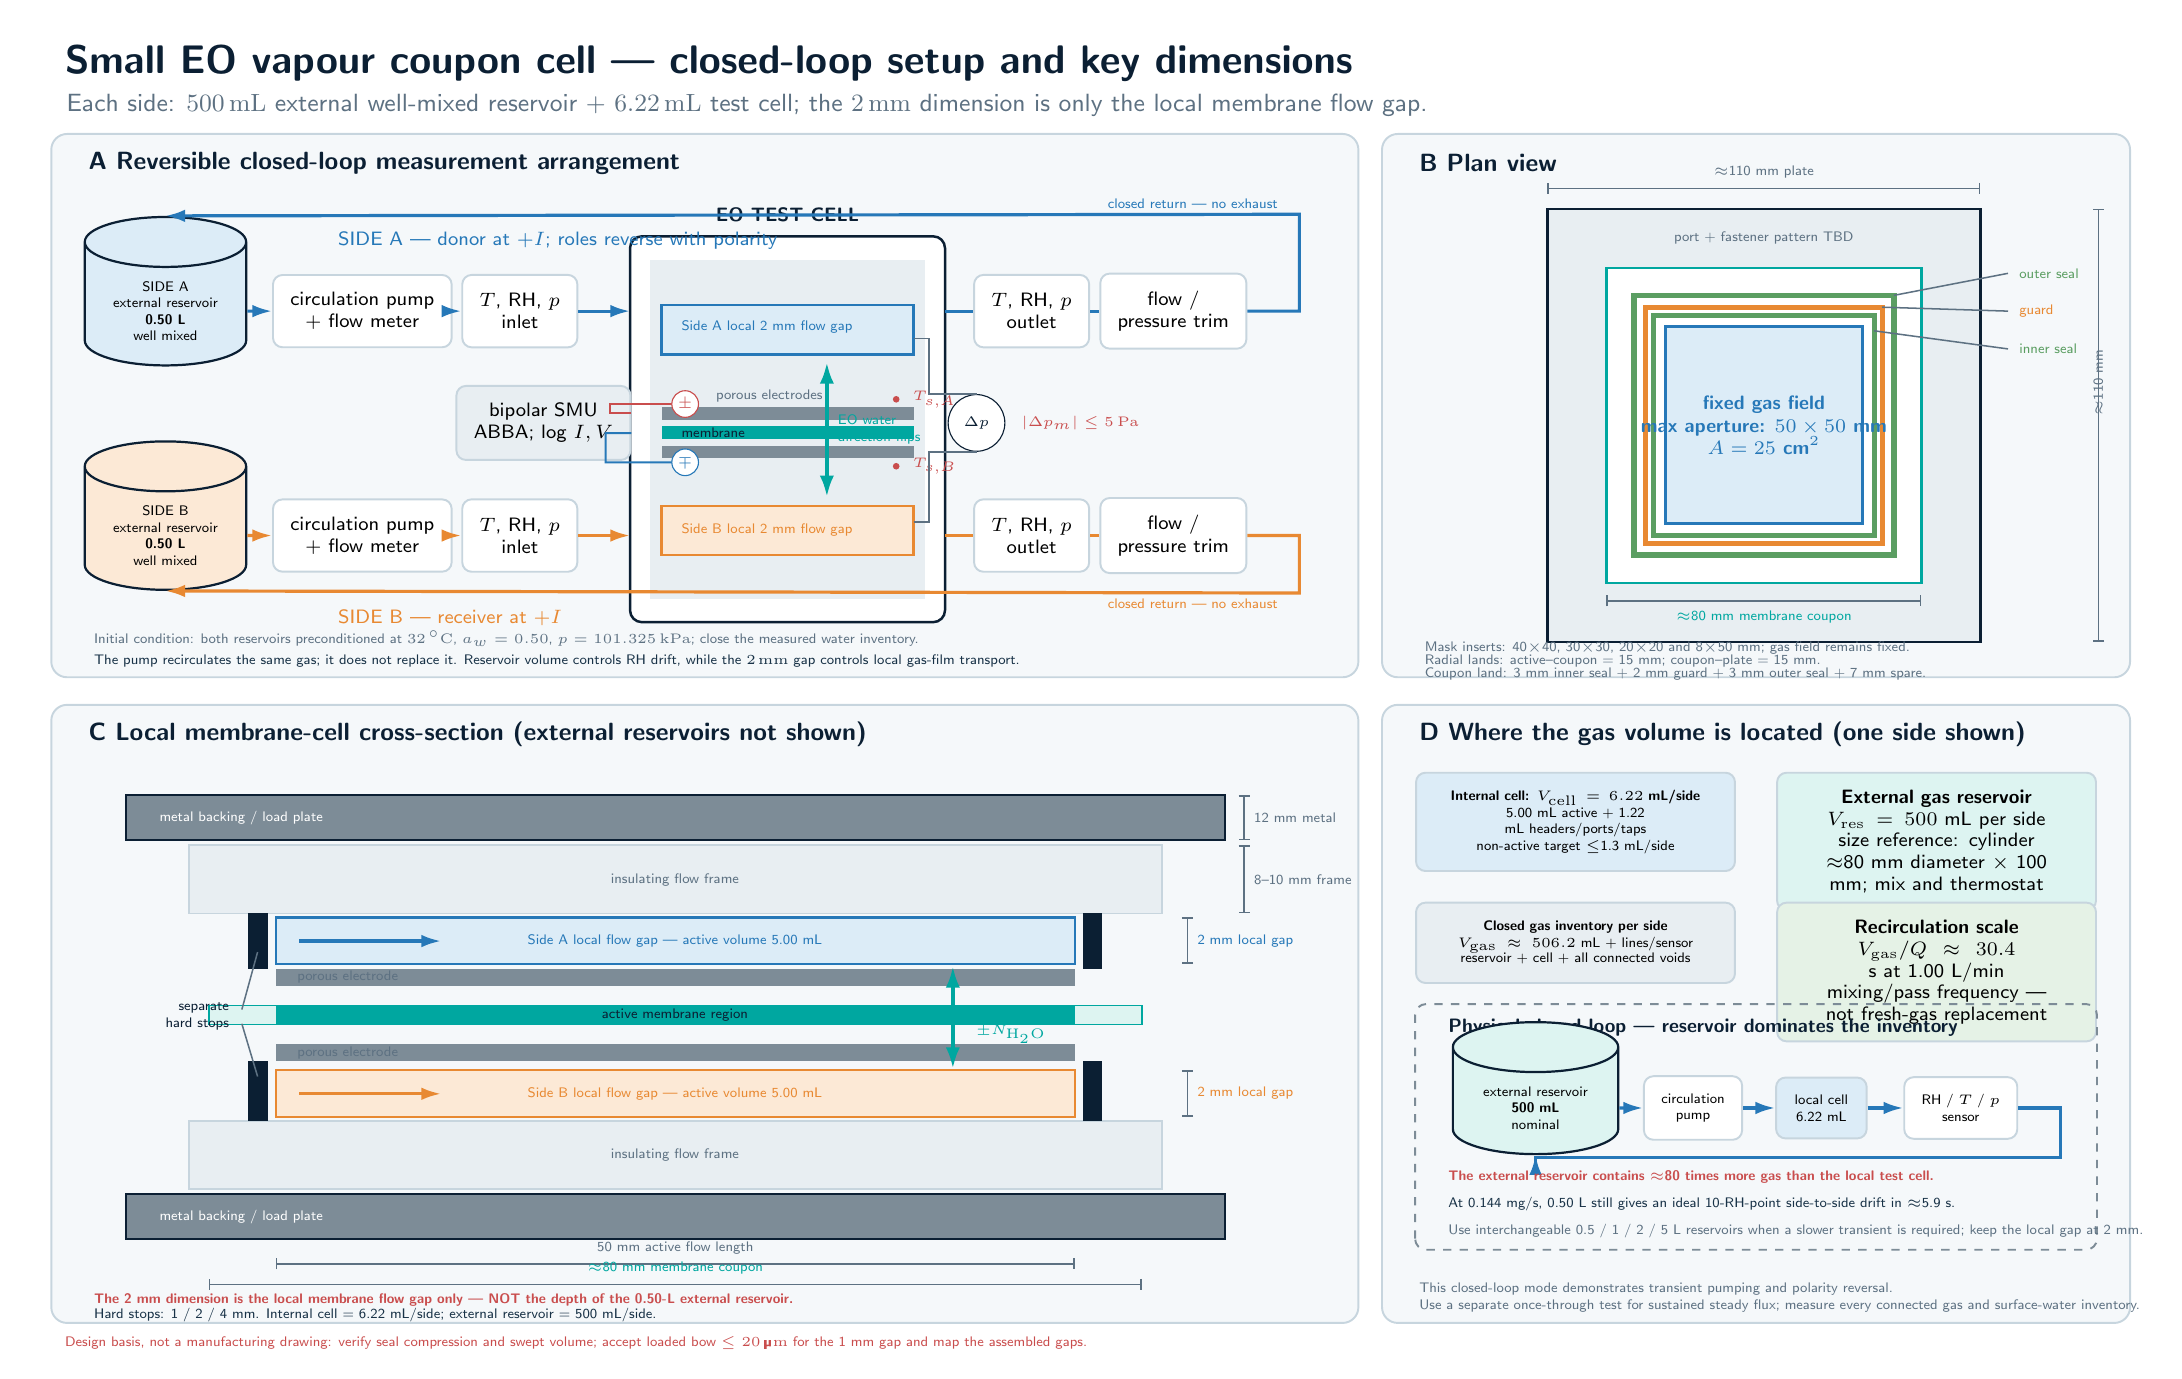
\begin{tikzpicture}[x=1cm,y=1cm]
  \path[use as bounding box] (0,0) rectangle (27,16.8);

  % Title
  \node[anchor=west, font=\sffamily\bfseries\Large, text=Navy]
    at (0.35,16.35) {Small EO vapour coupon cell --- closed-loop setup and key dimensions};
  \node[anchor=west, font=\sffamily\small, text=Slate]
    at (0.37,15.82) {Each side: \SI{500}{mL} external well-mixed reservoir + \SI{6.22}{mL} test cell; the \SI{2}{mm} dimension is only the local membrane flow gap.};

  % ---------------------------------------------------------------------------
  % Panel A: closed-loop setup
  % ---------------------------------------------------------------------------
  \draw[panel] (0.3,8.55) rectangle (16.9,15.45);
  \node[anchor=west, font=\sffamily\bfseries\small, text=Navy]
    at (0.65,15.08) {A  Reversible closed-loop measurement arrangement};

  \node[reservoir, fill=BlueLight] (resS) at (1.75,13.20)
    {SIDE A\\external reservoir\\\textbf{0.50 L}\\well mixed};
  \node[reservoir, fill=OrangeLight] (resR) at (1.75,10.35)
    {SIDE B\\external reservoir\\\textbf{0.50 L}\\well mixed};

  \node[box, minimum width=1.55cm, minimum height=0.82cm] (mfcS) at (4.25,13.20)
    {circulation pump\\+ flow meter};
  \node[box, minimum width=1.55cm, minimum height=0.82cm] (mfcR) at (4.25,10.35)
    {circulation pump\\+ flow meter};
  \draw[flow, Blue] (resS.east) -- (mfcS.west);
  \draw[flow, Orange] (resR.east) -- (mfcR.west);

  \node[box, minimum width=1.45cm, minimum height=0.92cm] (inS) at (6.25,13.20)
    {$T$, RH, $p$\\inlet};
  \node[box, minimum width=1.45cm, minimum height=0.92cm] (inR) at (6.25,10.35)
    {$T$, RH, $p$\\inlet};
  \draw[flow, Blue] (mfcS.east) -- (inS.west);
  \draw[flow, Orange] (mfcR.east) -- (inR.west);

  % Cell body
  \draw[rounded corners=1.5mm, draw=Navy, line width=0.9pt, fill=white]
    (7.65,9.25) rectangle (11.65,14.15);
  \node[anchor=south, font=\sffamily\bfseries\scriptsize, text=Navy]
    at (9.65,14.22) {EO TEST CELL};
  \fill[GreyLight] (7.9,9.55) rectangle (11.4,13.85);
  \fill[BlueLight] (8.05,12.65) rectangle (11.25,13.28);
  \draw[Blue, line width=0.8pt] (8.05,12.65) rectangle (11.25,13.28);
  \fill[OrangeLight] (8.05,10.10) rectangle (11.25,10.73);
  \draw[Orange, line width=0.8pt] (8.05,10.10) rectangle (11.25,10.73);
  \fill[Grey] (8.05,11.82) rectangle (11.25,11.98);
  \fill[Teal] (8.05,11.57) rectangle (11.25,11.74);
  \fill[Grey] (8.05,11.33) rectangle (11.25,11.49);
  \node[font=\sffamily\tiny, text=Blue, anchor=west] at (8.18,13.00) {Side A local 2 mm flow gap};
  \node[font=\sffamily\tiny, text=Orange, anchor=west] at (8.18,10.42) {Side B local 2 mm flow gap};
  \node[font=\sffamily\tiny, text=Navy, anchor=west] at (8.18,11.66) {membrane};
  \draw[waterrev] (10.15,12.55) -- node[right, align=left, font=\sffamily\tiny, text=Teal]
    {EO water\\direction flips} (10.15,10.84);

  % Bipolar electrical drive and local membrane-face temperature probes.
  \node[box, minimum width=1.35cm, minimum height=0.78cm, fill=GreyLight]
    (smu) at (6.55,11.78) {bipolar SMU\\ABBA; log $I,V$};
  \draw[Red, line width=0.75pt]
    ($(smu.east)+(0,0.13)$) -- (7.40,11.91) |- (8.20,12.02);
  \draw[Blue, line width=0.75pt]
    ($(smu.east)+(0,-0.13)$) -- (7.34,11.65) |- (8.20,11.28);
  \node[circle, draw=Red, text=Red, fill=white, inner sep=0.35mm,
    font=\sffamily\bfseries\tiny] at (8.35,12.02) {$\pm$};
  \node[circle, draw=Blue, text=Blue, fill=white, inner sep=0.35mm,
    font=\sffamily\bfseries\tiny] at (8.35,11.28) {$\mp$};
  \node[font=\sffamily\tiny, text=Slate, anchor=west] at (8.62,12.12) {porous electrodes};
  \fill[Red] (11.03,12.08) circle (1.2pt);
  \fill[Red] (11.03,11.23) circle (1.2pt);
  \node[font=\sffamily\tiny, text=Red, anchor=west] at (11.12,12.08) {$T_{s,A}$};
  \node[font=\sffamily\tiny, text=Red, anchor=west] at (11.12,11.23) {$T_{s,B}$};

  \draw[flow, Blue] (inS.east) -- (7.65,13.20);
  \draw[flow, Orange] (inR.east) -- (7.65,10.35);

  \node[box, minimum width=1.25cm, minimum height=0.92cm] (outS) at (12.75,13.20)
    {$T$, RH, $p$\\outlet};
  \node[box, minimum width=1.25cm, minimum height=0.92cm] (outR) at (12.75,10.35)
    {$T$, RH, $p$\\outlet};
  \draw[Blue, line width=1.15pt] (11.65,13.20) -- (outS.west);
  \draw[Orange, line width=1.15pt] (11.65,10.35) -- (outR.west);

  \node[box, minimum width=1.05cm, minimum height=0.72cm] (bpS) at (14.55,13.20) {flow /\\pressure trim};
  \node[box, minimum width=1.05cm, minimum height=0.72cm] (bpR) at (14.55,10.35) {flow /\\pressure trim};
  \draw[Blue, line width=1.15pt] (outS.east) -- (bpS.west);
  \draw[Orange, line width=1.15pt] (outR.east) -- (bpR.west);
  \draw[flow, Blue] (bpS.east) -- (16.15,13.20) -- (16.15,14.43) -- (resS.north);
  \draw[flow, Orange] (bpR.east) -- (16.15,10.35) -- (16.15,9.62) -- (resR.south);
  \node[anchor=east, font=\sffamily\tiny, text=Blue] at (16.00,14.57) {closed return --- no exhaust};
  \node[anchor=east, font=\sffamily\tiny, text=Orange] at (16.00,9.49) {closed return --- no exhaust};

  \node[circle, draw=Navy, fill=white, minimum size=0.72cm,
    font=\sffamily\bfseries\tiny, text=Navy] (dp) at (12.05,11.78) {$\Delta p$};
  \draw[leader] (11.25,12.85) -- (11.45,12.85) |- (dp.north);
  \draw[leader] (11.25,10.52) -- (11.45,10.52) |- (dp.south);
  \node[anchor=west, font=\sffamily\tiny, text=Red] at (12.5,11.78)
    {$|\Delta p_m|\leq\SI{5}{Pa}$};

  \node[anchor=west, font=\sffamily\scriptsize, text=Blue]
    at (3.82,14.10) {SIDE A --- donor at $+I$; roles reverse with polarity};
  \node[anchor=west, font=\sffamily\scriptsize, text=Orange]
    at (3.82,9.30) {SIDE B --- receiver at $+I$};
  \node[anchor=west, font=\sffamily\tiny, text=Slate]
    at (0.72,9.04) {Initial condition: both reservoirs preconditioned at \SI{32}{\celsius}, $a_w=0.50$, $p=\SI{101.325}{kPa}$; close the measured water inventory.};
  \node[anchor=west, font=\sffamily\tiny, text=Ink]
    at (0.72,8.76) {The pump recirculates the same gas; it does not replace it. Reservoir volume controls RH drift, while the \SI{2}{mm} gap controls local gas-film transport.};

  % ---------------------------------------------------------------------------
  % Panel B: plan dimensions
  % ---------------------------------------------------------------------------
  \draw[panel] (17.2,8.55) rectangle (26.7,15.45);
  \node[anchor=west, font=\sffamily\bfseries\small, text=Navy]
    at (17.55,15.08) {B  Plan view};

  \coordinate (pc) at (22.05,11.75);
  % Outer plate 110 mm
  \fill[GreyLight] (19.30,9.00) rectangle (24.80,14.50);
  \draw[Navy, line width=0.9pt] (19.30,9.00) rectangle (24.80,14.50);
  % Coupon 80 mm
  \fill[white] (20.05,9.75) rectangle (24.05,13.75);
  \draw[Teal, line width=0.8pt] (20.05,9.75) rectangle (24.05,13.75);
  % Seal / guard geometry: scaled from 66, 60, 56 and 50 mm
  \draw[Green, line width=2.0pt] (20.40,10.10) rectangle (23.70,13.40);
  \draw[Orange, line width=1.8pt] (20.55,10.25) rectangle (23.55,13.25);
  \draw[Green, line width=1.8pt] (20.65,10.35) rectangle (23.45,13.15);
  % Active aperture
  \fill[BlueLight] (20.80,10.50) rectangle (23.30,13.00);
  \draw[Blue, line width=1.0pt] (20.80,10.50) rectangle (23.30,13.00);
  \node[align=center, font=\sffamily\bfseries\scriptsize, text=Blue]
    at (22.05,11.75) {fixed gas field\\max aperture: $50\times50$ mm\\$A=25$ cm$^2$};

  % Exact port and fastener patterns are intentionally omitted.
  \node[font=\sffamily\tiny, text=Slate] at (22.05,14.13) {port + fastener pattern TBD};

  % Dimension lines
  \draw[dim] (19.30,14.76) -- node[above, font=\sffamily\tiny, text=Slate] {$\approx$110 mm plate} (24.80,14.76);
  \draw[dim] (26.30,9.00) -- node[right, rotate=90, font=\sffamily\tiny, text=Slate] {$\approx$110 mm} (26.30,14.50);
  \draw[dim] (20.05,9.52) -- node[below, font=\sffamily\tiny, text=Teal] {$\approx$80 mm membrane coupon} (24.05,9.52);
  \draw[leader] (23.70,13.40) -- (25.15,13.68);
  \node[anchor=west, font=\sffamily\tiny, text=Green] at (25.17,13.68) {outer seal};
  \draw[leader] (23.55,13.25) -- (25.15,13.20);
  \node[anchor=west, font=\sffamily\tiny, text=Orange] at (25.17,13.20) {guard};
  \draw[leader] (23.45,12.95) -- (25.15,12.72);
  \node[anchor=west, font=\sffamily\tiny, text=Green] at (25.17,12.72) {inner seal};
  \node[anchor=west, font=\sffamily\tiny, text=Slate]
    at (17.62,8.92) {Mask inserts: 40$\times$40, 30$\times$30, 20$\times$20 and 8$\times$50 mm; gas field remains fixed.};
  \node[anchor=west, font=\sffamily\tiny, text=Slate]
    at (17.62,8.75) {Radial lands: active--coupon = 15 mm; coupon--plate = 15 mm.};
  \node[anchor=west, font=\sffamily\tiny, text=Slate]
    at (17.62,8.59) {Coupon land: 3 mm inner seal + 2 mm guard + 3 mm outer seal + 7 mm spare.};

  % ---------------------------------------------------------------------------
  % Panel C: cross section
  % ---------------------------------------------------------------------------
  \draw[panel] (0.3,0.35) rectangle (16.9,8.20);
  \node[anchor=west, font=\sffamily\bfseries\small, text=Navy]
    at (0.65,7.82) {C  Local membrane-cell cross-section (external reservoirs not shown)};

  % Outer load plates
  \fill[Grey] (1.25,6.48) rectangle (15.20,7.05);
  \fill[Grey] (1.25,1.42) rectangle (15.20,1.99);
  \draw[Navy, line width=0.7pt] (1.25,6.48) rectangle (15.20,7.05);
  \draw[Navy, line width=0.7pt] (1.25,1.42) rectangle (15.20,1.99);
  \node[anchor=west, font=\sffamily\tiny, text=white] at (1.55,6.76) {metal backing / load plate};
  \node[anchor=west, font=\sffamily\tiny, text=white] at (1.55,1.70) {metal backing / load plate};

  % Insulating flow frames
  \fill[GreyLight] (2.05,5.55) rectangle (14.40,6.42);
  \fill[GreyLight] (2.05,2.05) rectangle (14.40,2.92);
  \draw[Line, line width=0.7pt] (2.05,5.55) rectangle (14.40,6.42);
  \draw[Line, line width=0.7pt] (2.05,2.05) rectangle (14.40,2.92);
  \node[font=\sffamily\tiny, text=Slate] at (8.22,5.98) {insulating flow frame};
  \node[font=\sffamily\tiny, text=Slate] at (8.22,2.48) {insulating flow frame};

  % Channels, electrodes, membrane
  \fill[BlueLight] (3.15,4.91) rectangle (13.30,5.50);
  \draw[Blue, line width=0.8pt] (3.15,4.91) rectangle (13.30,5.50);
  \fill[OrangeLight] (3.15,2.97) rectangle (13.30,3.56);
  \draw[Orange, line width=0.8pt] (3.15,2.97) rectangle (13.30,3.56);
  \fill[Grey] (3.15,4.63) rectangle (13.30,4.84);
  \fill[TealLight] (2.30,4.14) rectangle (14.15,4.38);
  \draw[Teal, line width=0.55pt] (2.30,4.14) rectangle (14.15,4.38);
  \fill[Teal] (3.15,4.14) rectangle (13.30,4.38);
  \fill[Grey] (3.15,3.68) rectangle (13.30,3.89);
  \node[font=\sffamily\tiny, text=Blue] at (8.22,5.20) {Side A local flow gap --- active volume 5.00 mL};
  \node[font=\sffamily\tiny, text=Orange] at (8.22,3.26) {Side B local flow gap --- active volume 5.00 mL};
  \node[font=\sffamily\tiny, text=Navy] at (8.22,4.26) {active membrane region};
  \node[anchor=west, font=\sffamily\tiny, text=Slate] at (3.30,4.74) {porous electrode};
  \node[anchor=west, font=\sffamily\tiny, text=Slate] at (3.30,3.78) {porous electrode};
  \draw[flow, Blue] (3.45,5.20) -- (5.25,5.20);
  \draw[flow, Orange] (3.45,3.26) -- (5.25,3.26);
  \draw[waterrev] (11.75,4.88) -- (11.75,3.58);
  \node[anchor=west, font=\sffamily\tiny, text=Teal] at (11.92,4.02)
    {$\pm N_{\mathrm{H_2O}}$};

  % Hard stops
  \fill[Navy] (2.80,4.84) rectangle (3.05,5.55);
  \fill[Navy] (13.40,4.84) rectangle (13.65,5.55);
  \fill[Navy] (2.80,2.92) rectangle (3.05,3.68);
  \fill[Navy] (13.40,2.92) rectangle (13.65,3.68);
  \node[anchor=east, align=right, font=\sffamily\tiny, text=Navy]
    at (2.68,4.24) {separate\\hard stops};
  \draw[leader] (2.72,4.33) -- (2.92,5.06);
  \draw[leader] (2.72,4.15) -- (2.92,3.48);

  % Cross-section dimensions
  \draw[dim] (3.15,1.10) -- node[above, font=\sffamily\tiny, text=Slate]
    {50 mm active flow length} (13.30,1.10);
  \draw[dim] (2.30,0.84) -- node[above, font=\sffamily\tiny, text=Teal]
    {$\approx$80 mm membrane coupon} (14.15,0.84);
  \draw[dim] (14.73,4.91) -- node[right, font=\sffamily\tiny, text=Blue] {2 mm local gap} (14.73,5.50);
  \draw[dim] (14.73,2.97) -- node[right, font=\sffamily\tiny, text=Orange] {2 mm local gap} (14.73,3.56);
  \draw[dim] (15.45,5.55) -- node[right, font=\sffamily\tiny, text=Slate] {8--10 mm frame} (15.45,6.42);
  \draw[dim] (15.45,6.48) -- node[right, font=\sffamily\tiny, text=Slate] {12 mm metal} (15.45,7.05);
  \node[anchor=west, font=\sffamily\bfseries\tiny, text=Red]
    at (0.72,0.64) {The 2 mm dimension is the local membrane flow gap only --- NOT the depth of the 0.50-L external reservoir.};
  \node[anchor=west, font=\sffamily\tiny, text=Ink]
    at (0.72,0.45) {Hard stops: 1 / 2 / 4 mm. Internal cell = 6.22 mL/side; external reservoir = 500 mL/side.};

  % ---------------------------------------------------------------------------
  % Panel D: physical location of the gas inventory
  % ---------------------------------------------------------------------------
  \draw[panel] (17.2,0.35) rectangle (26.7,8.20);
  \node[anchor=west, font=\sffamily\bfseries\small, text=Navy]
    at (17.55,7.82) {D  Where the gas volume is located (one side shown)};

  \node[box, anchor=north west, minimum width=4.05cm, minimum height=1.08cm,
    fill=BlueLight, text width=3.55cm, font=\sffamily\tiny] at (17.62,7.35)
    {\textbf{Internal cell: $V_{\rm cell}=6.22$ mL/side}\\
     5.00 mL active + 1.22 mL headers/ports/taps\\
     non-active target $\leq$1.3 mL/side};
  \node[box, anchor=north east, minimum width=4.05cm, minimum height=1.08cm,
    fill=TealLight, text width=3.55cm] at (26.28,7.35)
    {\textbf{External gas reservoir}\\$V_{\rm res}=500$ mL per side\\[-0.2ex]
     \scriptsize size reference: cylinder $\approx$80 mm diameter $\times$ 100 mm; mix and thermostat};
  \node[box, anchor=north west, minimum width=4.05cm, minimum height=1.02cm,
    fill=GreyLight, text width=3.55cm, font=\sffamily\tiny] at (17.62,5.70)
    {\textbf{Closed gas inventory per side}\\$V_{\rm gas}\approx506.2$ mL + lines/sensor\\[-0.2ex]
     reservoir + cell + all connected voids};
  \node[box, anchor=north east, minimum width=4.05cm, minimum height=1.02cm,
    fill=GreenLight, text width=3.55cm] at (26.28,5.70)
    {\textbf{Recirculation scale}\\$V_{\rm gas}/Q\approx30.4$ s at 1.00 L/min\\[-0.2ex]
     \scriptsize mixing/pass frequency --- not fresh-gas replacement};

  \draw[dashed, rounded corners=1.4mm, draw=Grey, line width=0.7pt]
    (17.62,1.28) rectangle (26.28,4.40);
  \node[anchor=west, font=\sffamily\bfseries\scriptsize, text=Navy]
    at (17.92,4.10) {Physical closed loop --- reservoir dominates the inventory};

  \node[reservoir, fill=TealLight, minimum width=2.10cm, minimum height=1.20cm]
    (dres) at (19.15,3.08) {external reservoir\\\textbf{500 mL}\\nominal};
  \node[box, minimum width=1.15cm, minimum height=0.66cm, font=\sffamily\tiny]
    (dpump) at (21.15,3.08) {circulation\\pump};
  \node[box, minimum width=1.15cm, minimum height=0.66cm, fill=BlueLight,
    font=\sffamily\tiny] (dcell) at (22.78,3.08) {local cell\\6.22 mL};
  \node[box, minimum width=1.30cm, minimum height=0.66cm, font=\sffamily\tiny]
    (dsensor) at (24.55,3.08) {RH / $T$ / $p$\\sensor};
  \draw[flow, Blue] (dres.east) -- (dpump.west);
  \draw[flow, Blue] (dpump.east) -- (dcell.west);
  \draw[flow, Blue] (dcell.east) -- (dsensor.west);
  \draw[flow, Blue] (dsensor.east) -- (25.82,3.08) -- (25.82,2.45) -- (19.15,2.45) -- (dres.south);

  \node[anchor=west, font=\sffamily\bfseries\tiny, text=Red] at (17.92,2.20)
    {The external reservoir contains $\approx$80 times more gas than the local test cell.};
  \node[anchor=west, font=\sffamily\tiny, text=Ink] at (17.92,1.86)
    {At 0.144 mg/s, 0.50 L still gives an ideal 10-RH-point side-to-side drift in $\approx$5.9 s.};
  \node[anchor=west, font=\sffamily\tiny, text=Slate] at (17.92,1.52)
    {Use interchangeable 0.5 / 1 / 2 / 5 L reservoirs when a slower transient is required; keep the local gap at 2 mm.};

  \node[anchor=west, font=\sffamily\tiny, text=Slate]
    at (17.55,0.78) {This closed-loop mode demonstrates transient pumping and polarity reversal.};
  \node[anchor=west, font=\sffamily\tiny, text=Slate]
    at (17.55,0.57) {Use a separate once-through test for sustained steady flux; measure every connected gas and surface-water inventory.};

  \node[anchor=west, font=\sffamily\tiny, text=Red]
    at (0.35,0.10) {Design basis, not a manufacturing drawing: verify seal compression and swept volume; accept loaded bow $\leq\SI{20}{\micro\metre}$ for the 1 mm gap and map the assembled gaps.};

\end{tikzpicture}
\end{document}
